\documentclass[10pt]{article}
\setlength{\topmargin}{0in} % top margin is .5 in
\setlength{\oddsidemargin}{0in} % left margin is 1 in on right pages
\setlength{\evensidemargin}{0in} % same for left pages, 2-sided document
\setlength{\textwidth}{4in} % leaves 1 in for right margin
\setlength{\textheight}{6in} 


\usepackage{graphicx}
\usepackage{geometry}
\usepackage{amsmath}
\usepackage{microtype}
\usepackage{booktabs}
\usepackage{amssymb}

\begin{document}
\textbf{Figure 1}\\
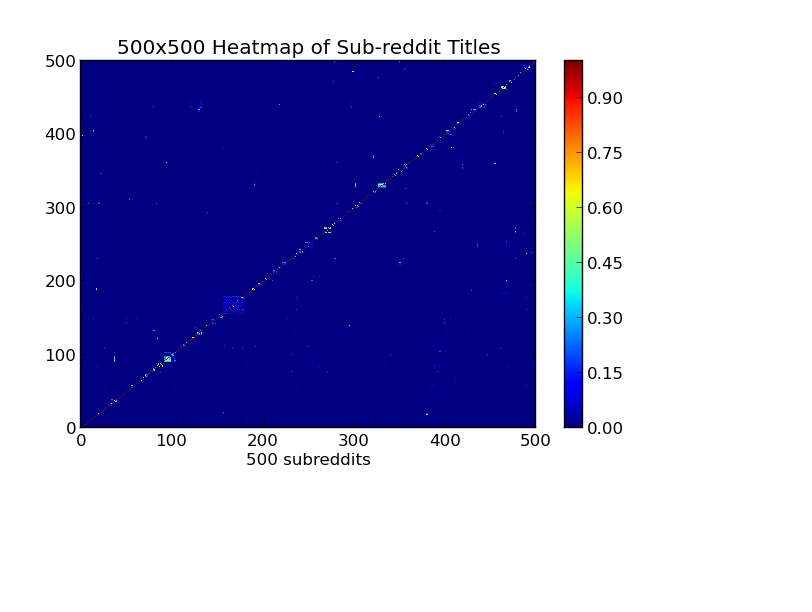
\includegraphics[scale=0.7]{500Heatmap.png}\\
The heatmap of a portion of the 2500x2500 Title similarity matrix (from 500-800).\\
There are patches on the diagonal and sparse scatters everywhere else.\\
\pagebreak\\
\textbf{Figure 2}\\
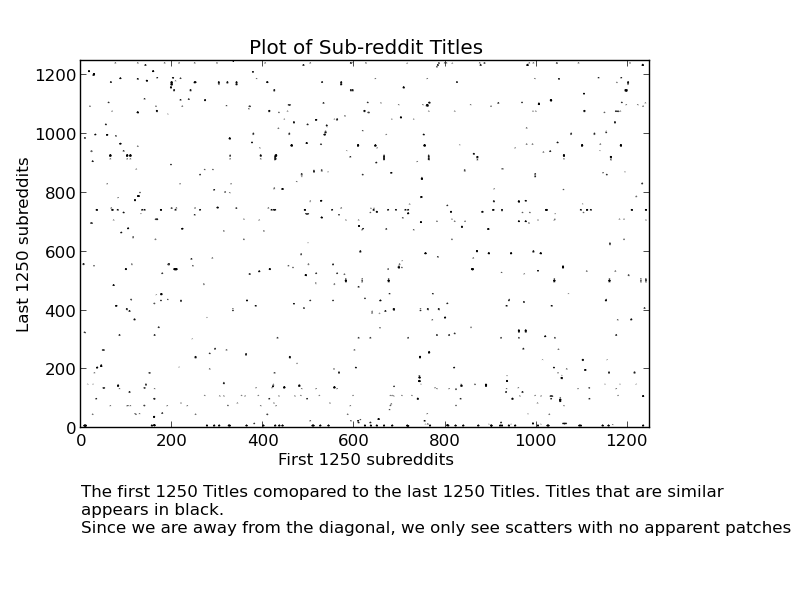
\includegraphics[scale=0.45]{Title12501.png} 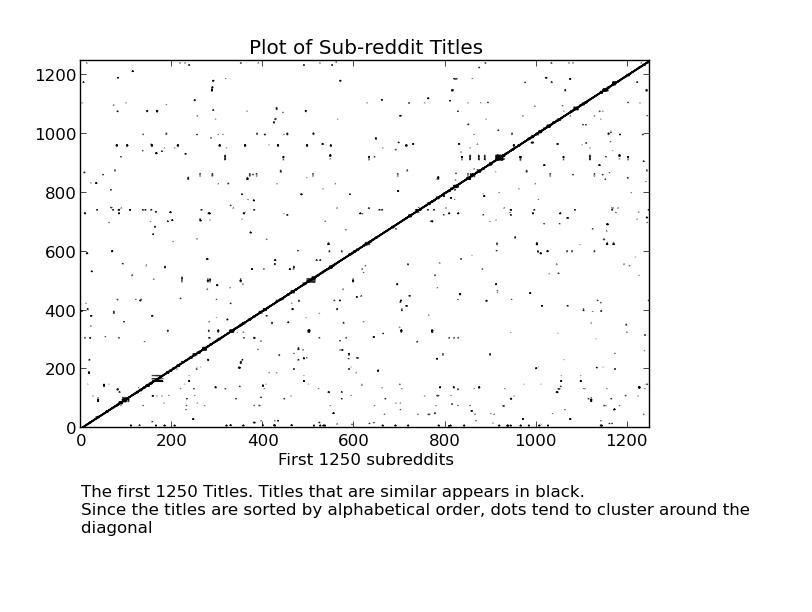
\includegraphics[scale=0.45]{Title1250.png}\\
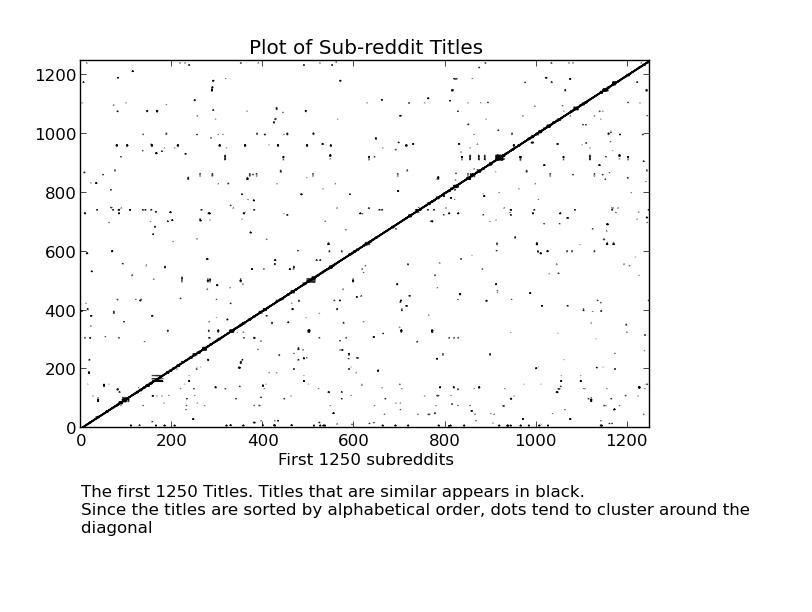
\includegraphics[scale=0.45]{Title1250.png} 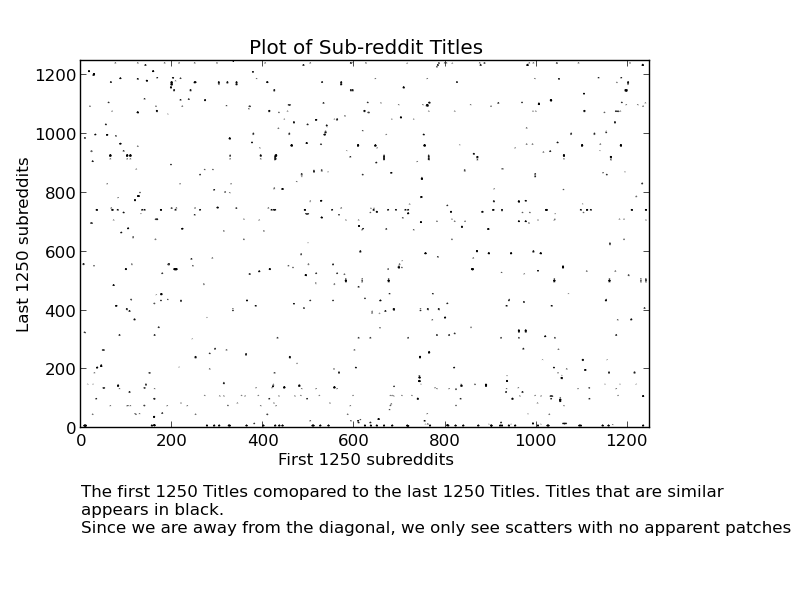
\includegraphics[scale=0.45]{Title12501.png}\\
A full view of the title similarity matrix, divided into four regions. \\
\pagebreak\\
\textbf{Figure 3}\\
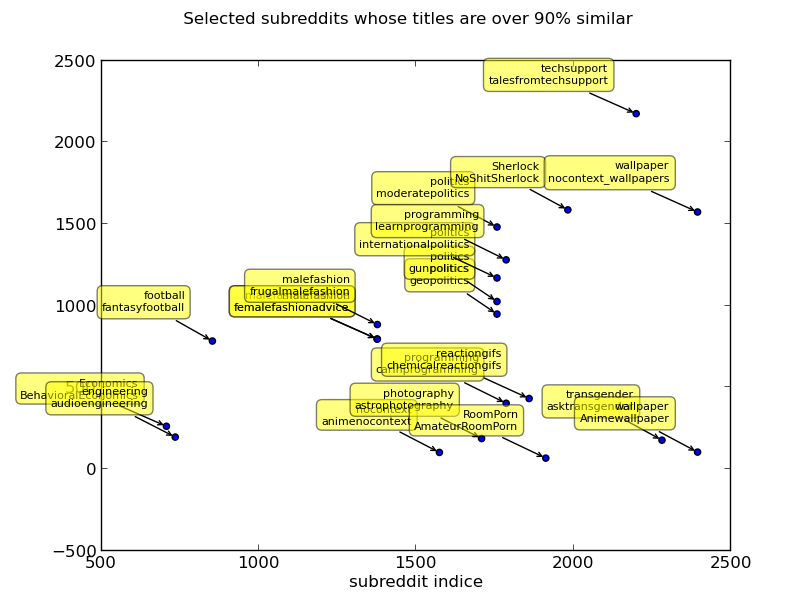
\includegraphics[scale=0.7]{TItle90.png}\\
Subreddits that are more than 90 percent similar to each others, with corresponding names attached.\\ 
\pagebreak\\
\textbf{Figure 4}\\
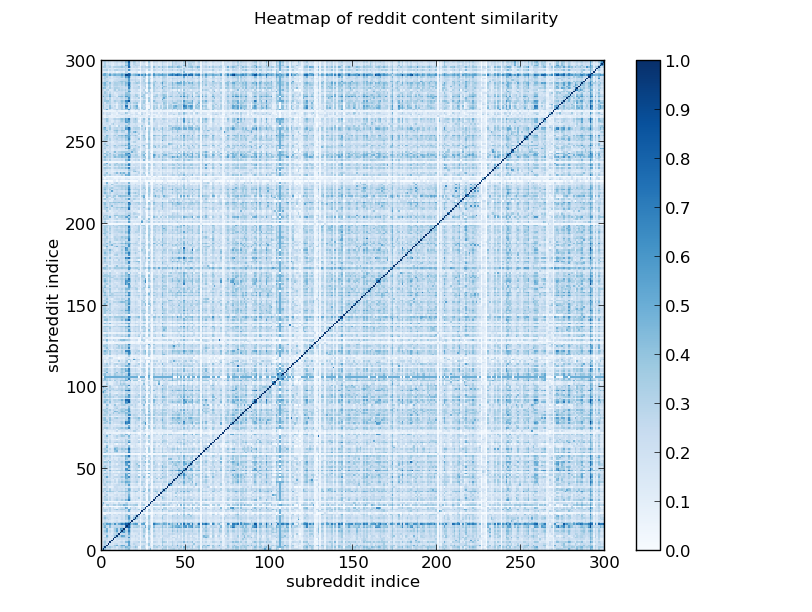
\includegraphics[scale=0.45]{HeatmapContent} 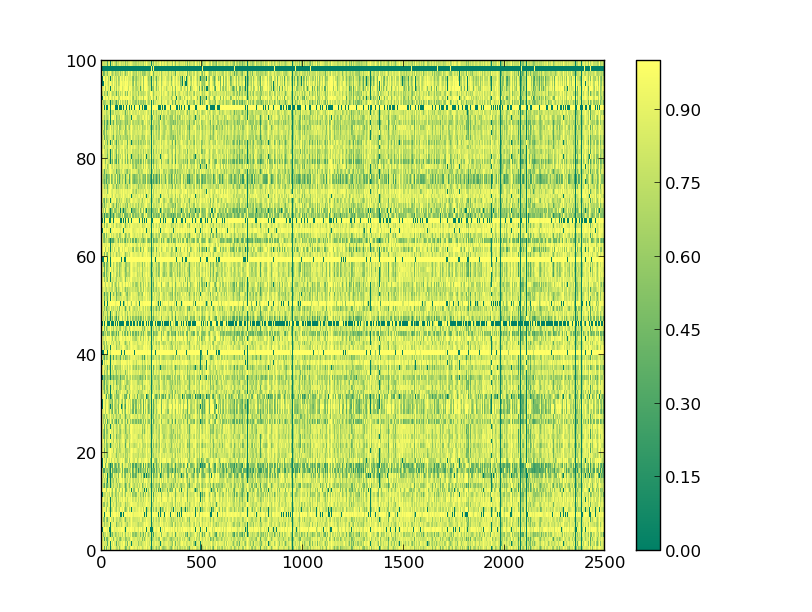
\includegraphics[scale=0.45]{TF100.png}\\
Left: a 300x300 region of the word-count similarity matrix. It has a large area of lightblue, only dark patches along the diagonal, implying most subreddits are distinct.\\
\linebreak
Right: a 100x1250 strip of the TFIDF-similarity matrix that aims to compare the similarity between any two given subreddits. It shows a high portion of yellow, indicating subreddits are quiet alike.\\
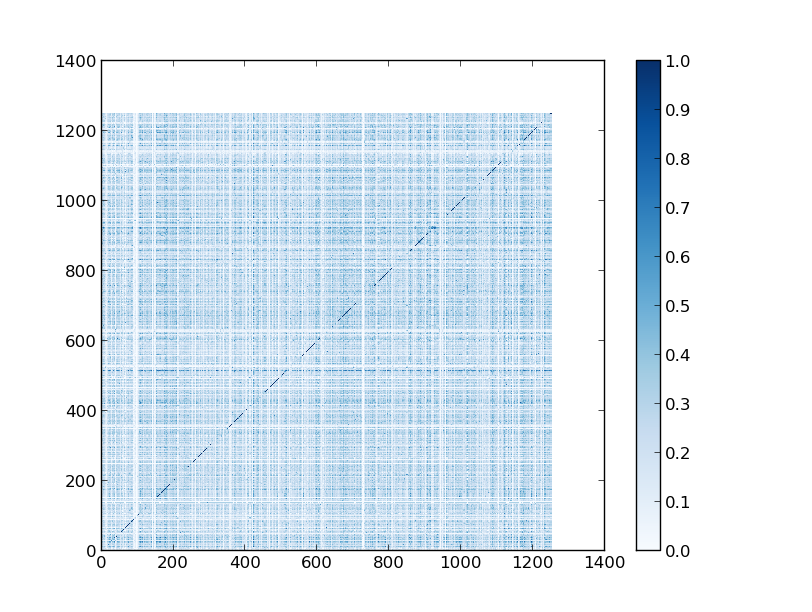
\includegraphics[scale=0.5]{W1250}\\ 
The same heatmap of content similarity computed base on word counts, at a large scale (1250x1250). \\
\pagebreak\\
\textbf{Figure 5}\\
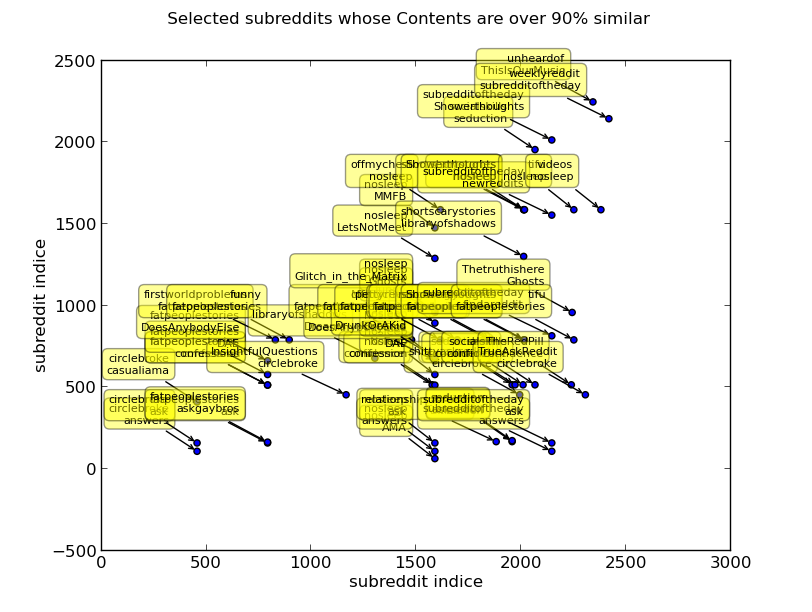
\includegraphics[scale=0.7]{content90}\\
A plot of subreddits whose contents are more than 90 percent similar to each other.\\
Note that several subreddits are similar to more than one other subreddits, therefore, appearing more than once.\\
\pagebreak\\
\textbf{Figure 6}\\
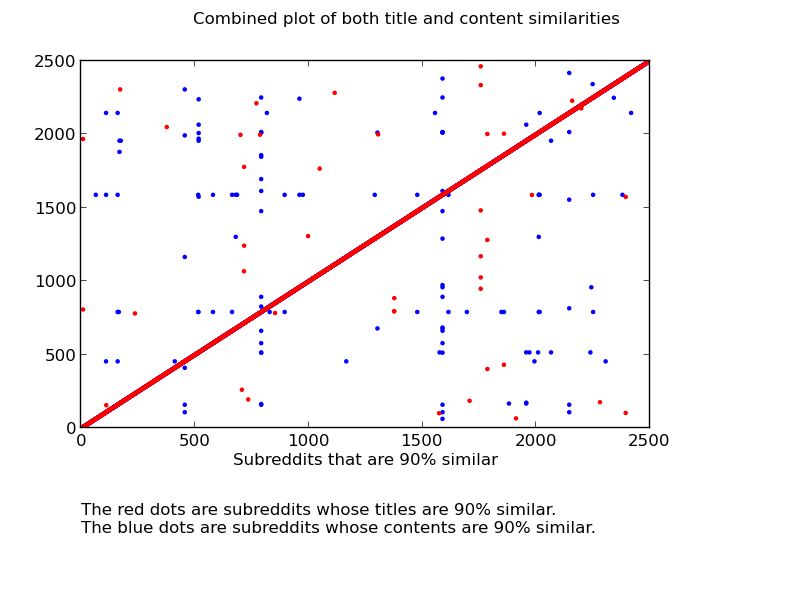
\includegraphics[scale=0.7]{match}\\
Subreddits who are 90 percent alike in title and 90 percent alike in content plotted on top of each other.\\
Subreddits who are similar in title tend to be similar in content, but subreddits that are similar in content may not have the same title as there are more blue dots than red dots.\\


\end{document}